\documentclass [a4paper, 11pt] {article}

%document configuration
\newcommand{\courseName}{Machine Learning in Graphics \& Vision}
\newcommand{\termYear}{Summer Term 2020}
\newcommand{\homeworkNum}{2}
\newcommand{\studentOne}{Driton Goxhufi}
\newcommand{\studentTwo} {Damir Ravlija}
\newcommand{\matrikelNrStOne}{4233242}
\newcommand{\matrikelNrStTwo}{5503184}
\newcommand{\mailStOne}{driton.goxhufi@student.uni-tuebingen.de}
\newcommand{\mailStTwo}{damir.ravlija@student.uni-tuebingen.de}

%packages
\usepackage [english] {babel}
\usepackage [T1] {fontenc}
\usepackage [utf8] {inputenc}
\usepackage {graphicx}
\usepackage {subcaption}
\usepackage {amsmath}
\usepackage {amssymb}
\usepackage {amstext}
\usepackage {amsthm}
\usepackage {listings}
\usepackage {tikz}
\usepackage[
pdftex,
pdfauthor={Goxhufi, Driton; Ravlija, Damir},
pdftitle={MLGV - Exercise \homeworkNum Submission},
pdfsubject={Machine Learning in Graphics \& Vision Homework}
]{hyperref}

\usepackage[a4paper,lmargin={2cm},rmargin={2cm},tmargin={3.5cm},bmargin = {2.5cm},headheight = {4cm}]{geometry}

\usepackage[shortlabels]{enumitem}
\usepackage{lastpage}
\usepackage{fancyhdr}

\usepackage{lipsum}
\usepackage{ifthen}

\pagestyle{fancy}



%other config
\renewcommand{\v}[1]{\boldsymbol{#1}}
\newcommand{\mat}[1]{\boldsymbol{#1}}
\newcommand{\m}[1]{\begin{pmatrix}#1\end{pmatrix}}
\newcommand{\tr}[2]{{}^{#1}T_{#2}}
\graphicspath{{./images/}}


\lhead{\begin{tabular}{l}
		\courseName\\
		\termYear \\
		Exercise \homeworkNum
\end{tabular}}
\rhead{\begin{tabular}{lr}
		\studentOne & \matrikelNrStOne \\
		\studentTwo & \matrikelNrStTwo \\
\end{tabular}}

\begin{document}
	
\title{\vspace{-1.5cm}\textbf{Exercise \homeworkNum} \\ 
	\courseName}
\author{\begin{tabular}{lcr}
		\studentOne & \matrikelNrStOne & \href{mailto:\mailStOne}{\mailStOne} \\
		\studentTwo & \matrikelNrStTwo & \href{mailto:\mailStTwo}{\mailStTwo} 
\end{tabular}}	
\date{}
\maketitle


\section{Task 1}
\begin{enumerate}
\item[(a)]
Classification accuracy of the initialized model on the test dataset is $0.5$


\item[(b)]
Loss of the initialized model is $0.7149616252170096$.

\item[(c)]
In the first step of derivation we use the chain rule and the fact that $f_{\v{w}}'(x) = f_{\v{w}}(x)(1-f_{\v{w}}(x)$.
\begin{align*}
\frac{\partial L(\v{x}, t, \v{w})}{\partial \v{w}} &\stackrel{(\ref{eq:c})}{=} \frac{1}{N}\sum_{n=1}^{N}\left[-t_n \frac{1}{f_{\v{w}}(\v{x}_n)}f_{\v{w}}(\v{x}_n)(1-f_{\v{w}}(\v{x}_n))\v{x}_n + (1-t_n)\frac{1}{1-f_{\v{w}}(\v{x_n})}f_{\v{w}}(\v{x}_n)(1-f_{\v{w}}(\v{x}_n))\v{x}_n \right] \\
&= \frac{1}{N}\sum_{n=1}^{N}\left[-t_n(1-f_{\v{w}}(\v{x}_n))\v{x}_n + (1-t_n)f_{\v{w}}(\v{x}_n)\v{x}_n \right] \\
&= \frac{1}{N}\sum_{n=1}^{N}\left[(-t_n + t_n f_{\v{w}}(\v{x}_n) + f_{\v{w}}(\v{x}_n) - t_nf_{\v{w}}(\v{x}_n))\v{x}_n\right] \\
&= \frac{1}{N}\sum_{n=1}^{N}\left[ f_{\v{w}}(\v{x}_n) - t_n\right]\v{x}_n
\end{align*}

\begin{enumerate}
	\item[(1)]\label{eq:c} 
	\begin{align*}
	\frac{\partial f_{\v{w}}(x)}{\partial x} &= \frac{\partial}{\partial x}\left(\frac{1}{1 + e^{-\v{w}^{T}\v{x}}}\right) = \frac{e^{-\v{w}^{T}\v{x}}}{{(1 + e^{-\v{w}^{T}\v{x}})}^2} = \frac{1 + e^{-\v{w}^{T}\v{x}} - 1}{{(1 + e^{-\v{w}^{T}\v{x}})}^2} = \frac{1}{{(1 + e^{-\v{w}^{T}\v{x}})}} - \frac{1}{{(1 + e^{-\v{w}^{T}\v{x}})}^2} \\
	&= \frac{1}{{(1 + e^{-\v{w}^{T}\v{x}})}} \left(1 - \frac{1}{{(1 + e^{-\v{w}^{T}\v{x}})}}\right) = f_{\v{w}}(\v{w}^{T}\v{x})(1 - f_{\v{w}}(\v{w}^{T}\v{x}))
	\end{align*}
\end{enumerate}

\bigskip
\bigskip
\bigskip

After $1,000$ iterations the loss and accuracy of the model are:

	\qquad loss $= 0.3868595564299156$
	
	\qquad accuracy $= 0.83$



	
\item[(d)]
Since $f_{\v{w}}$ represents the class posterior probability $p(c_1|\v{x})$, the loss is minimal for $t = 1$ when this probability is the highest (i.e. $f_{\v{w}} = 1$). As the confidence of the model decreases, the loss function grows up to infinity which corresponds to the case when the model is confident in the wrong class, i.e. assigns $f_{\v{w}} = 0$ (see Figure (\ref{fig:1}).  

On the other hand, if the label $t = 0$, the loss is minimized when $p(c_2|\v{x}) = 1 - p(c_1|\v{x}) = 1 - f_{\v{w}}$ is maximized which is achieved when $f_{\v{w}} = 0$. The loss is higher when the model assigns higher probability to the other class, and grows to infinity as $f_{\v{w}}$ nears 1. 

\begin{figure}[!h]
	\centering
	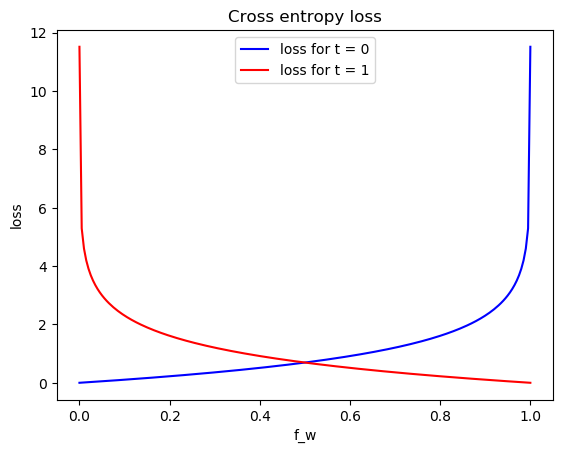
\includegraphics[width=0.8\textwidth]{img/2_1_d.png}
	\caption{Plot of results from task (d)}
	\label{fig:1}
\end{figure}

\item[(e)]
We observe that the lower the learning rate is, the increase in accuracy and loss decrease are slower but more stable over time. Even after $1,000$ iterations, smaller learning rates show increasing accuracy and decreasing loss trends, which implies that they would benefit from more iterations. Optimal learning rate that shows the best combination of stability and convergence speed is $0.1$. Both loss and accuracy achieve the best values when the learning rate is set to $0.1$.  

In the extreme case of learning rate set to 1, both loss and accuracy are extremely unstable. This instability probably arises from overly large steps that the gradient descent makes and which causes it to overstep the minima. Conversely, in case of the smallest learning rate $0.0001$ the accuracy of the model starts increasing only after around $200$ iterations.

\begin{figure}[!h]
	\centering
	\begin{subfigure}{0.4\textwidth}
		\centering
		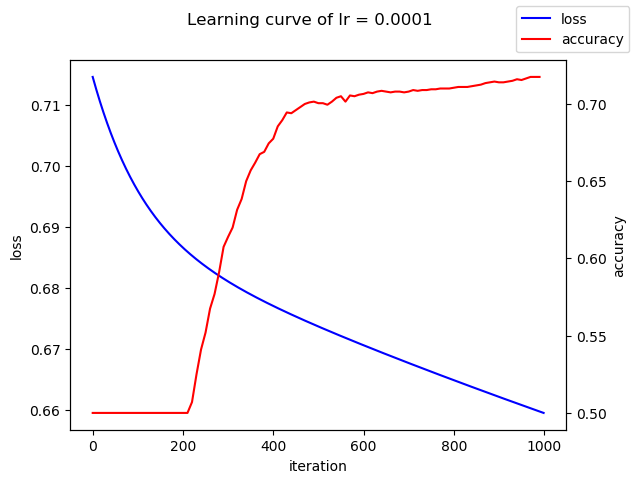
\includegraphics[width=\textwidth]{img/2_1_e_0-0001.png}
		\caption{Learning rate set to $0.0001$}
		\label{fig:2a}
	\end{subfigure}
	\begin{subfigure}{0.4\textwidth}
		\centering
		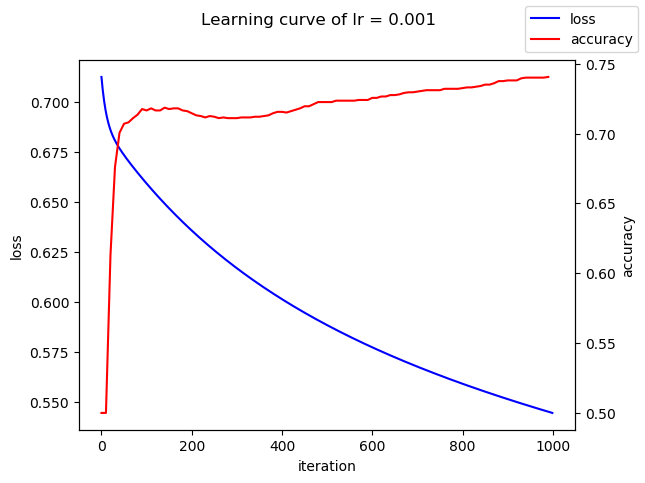
\includegraphics[width=\textwidth]{img/2_1_e_0-001.png}
		\caption{Learning rate set to $0.001$}
		\label{fig:2b}
	\end{subfigure}
	\begin{subfigure}{0.4\textwidth}
		\centering
		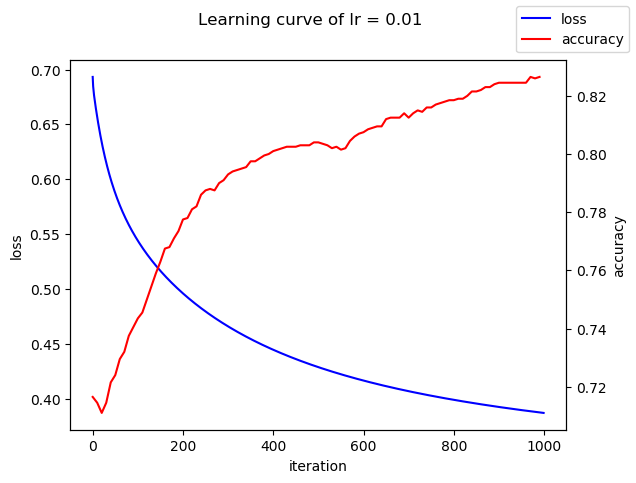
\includegraphics[width=\textwidth]{img/2_1_e_0-01.png}
		\caption{Learning rate set to $0.01$}
		\label{fig:2c}
	\end{subfigure}
	\begin{subfigure}{0.4\textwidth}
		\centering
		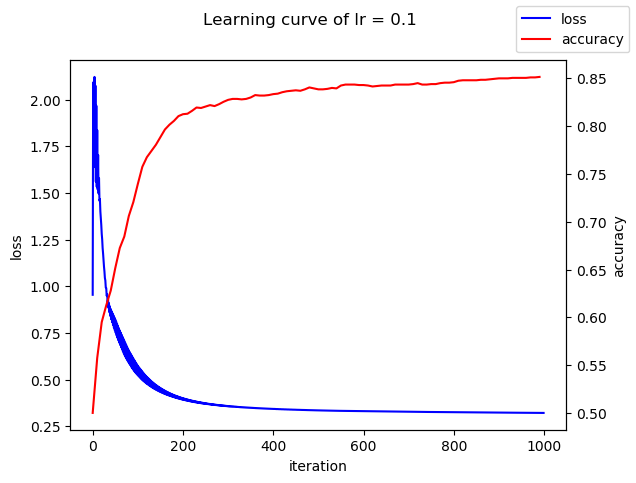
\includegraphics[width=\textwidth]{img/2_1_e_0-1.png}
		\caption{Learning rate set to $0.1$}
		\label{fig:2d}
	\end{subfigure}
	\begin{subfigure}{0.4\textwidth}
		\centering
		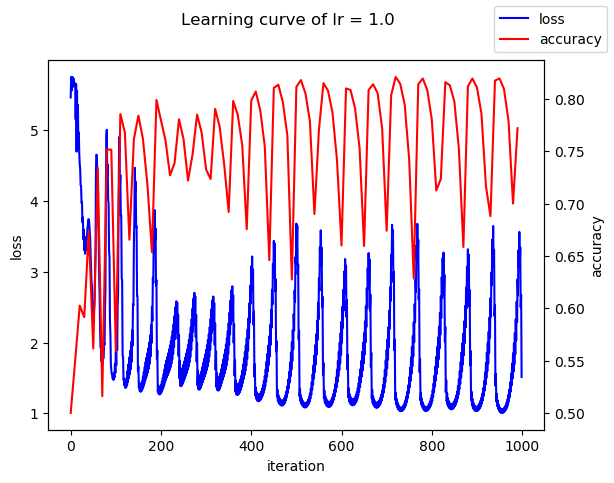
\includegraphics[width=\textwidth]{img/2_1_e_1-0.png}
		\caption{Learning rate set to $1$}
		\label{fig:2e}
	\end{subfigure}
	\caption{Plot of results from task (e)}
	\label{fig:2}
\end{figure}

\item[(f)]
\begin{figure}[!h]
	\centering
	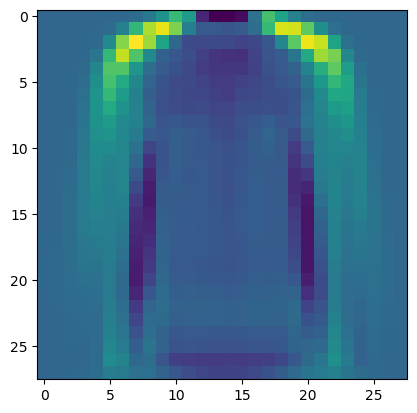
\includegraphics[width=0.8\textwidth]{img/2_1_f.png}
	\caption{Task f part 1}
	\label{fig:task-f}
\end{figure}

\begin{figure}[!h]
	\centering
	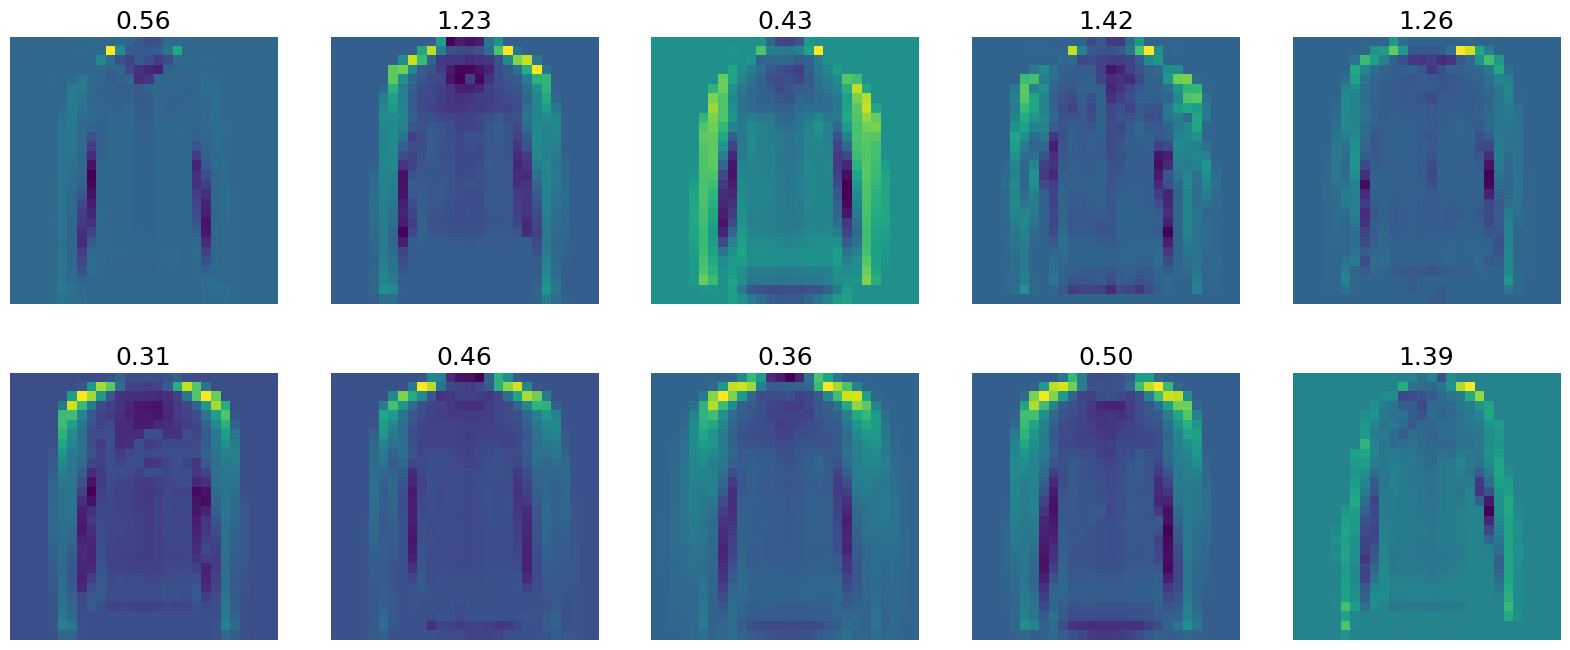
\includegraphics[width=0.8\textwidth]{img/2_1_f_1.png}
	\caption{Task f part 2}
	\label{fig:task-f-2}
\end{figure}


\item[(g)]
Inference step of this learning approach is more efficient than the nearest neighbors search which has to find the $k$ nearest neighbors. Another advantage of this learning approach is that it returns the probability of how confident it is that the value belongs to a certain class.

\end{enumerate}
	
\end{document}

